\documentclass{beamer}

\mode<presentation> {
    \usetheme{Prague}
    \setbeamercovered{transparent}
}

\usepackage{ucs}
\usepackage[utf8]{inputenc}
\usepackage[czech]{babel}
\usepackage{palatino}
\usepackage{graphicx}
\usepackage{epstopdf}

\title{E-puck knihovna pro Python}
\author{David Marek}
\institute[MFF UK]{Univerzita Karlova v Praze}
\date{5.~4.~2011}

\begin{document}

\begin{frame}
    \titlepage
\end{frame}

\begin{frame}
    \frametitle{Osnova}
    \tableofcontents
\end{frame}

\section{Představení e-puck robota}

\subsection{Úvod}

\begin{frame}
    \frametitle{E-Puck}
    \begin{columns}
        \begin{column}{.6\textwidth}
            \begin{itemize}
                \item Ecole Polytechnique Fédérale de Lausanne
                \item Miniaturní robot (průměr 75mm)
                \item Opensource hardware
                \item Spousta senzorů
                \item Bluetooth komunikace
                \item Dostupný (v labu)
            \end{itemize}
        \end{column}

        \begin{column}{.4\textwidth}
            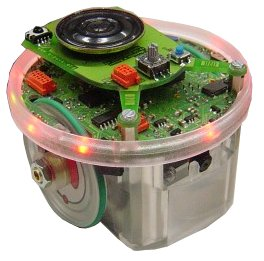
\includegraphics[scale=0.4]{e-puck.jpg}
        \end{column}
    \end{columns}
\end{frame}

\subsection{Senzory a akční členy}

\begin{frame}
    \frametitle{Senzory a akční členy}
    \begin{itemize}
        \item Kamera (640x480)
        \item IR senzory (proximity / ambient light)
        \item Akcelerometr (3D)
        \item Mikrofony
        \item LED
        \item Krokové motory
        \item Speaker
    \end{itemize}
\end{frame}

\begin{frame}
    \frametitle{Kamera}
    \begin{columns}
        \begin{column}{.7\textwidth}
            \begin{itemize}
                \item Rozlišení 640x480
                \item Dva režimy: RGB565 / barvy šedi
                \item Příliš velké fotky pro zpracování v robotovi
                \item Řešení problémů s pamětí:
                    \begin{itemize}
                        \item Prokládání
                        \item Změna formátu fotografie
                    \end{itemize}
                \item Reálně jde získat:
                    \begin{itemize}
                        \item 40x40 barevně
                        \item 55x55 černobíle
                        \item Lineární kamera
                    \end{itemize}
            \end{itemize}
        \end{column}

        \begin{column}[c]{.3\textwidth}
            \begin{center}
                \hspace{-2cm}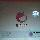
\includegraphics{fotka1.jpg}\\
                \vspace{0.3cm}
                \hspace{-2cm}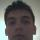
\includegraphics{fotka2.jpg}\\
                \vspace{0.3cm}
                \hspace{-2cm}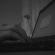
\includegraphics{fotka3.jpg}\\
                \vspace{0.3cm}
                \hspace{-2cm}
\includegraphics[scale=0.4]{fotka4.jpg}
            \end{center}
        \end{column}
    \end{columns}
\end{frame}

\begin{frame}
    \frametitle{IR senzory}
    \begin{columns}
        \begin{column}{0.6\textwidth}
            \begin{itemize}
                \item 8 senzorů po obvodu
                \item Dva režimy:
                    \begin{itemize}
                        \item Aktivní -- rozeznávání překážek
                        \item Pasivní -- intenzita světla
                    \end{itemize}
                \item Překážky do $\sim$ 4cm
            \end{itemize}
        \end{column}

        \begin{column}{0.4\textwidth}
            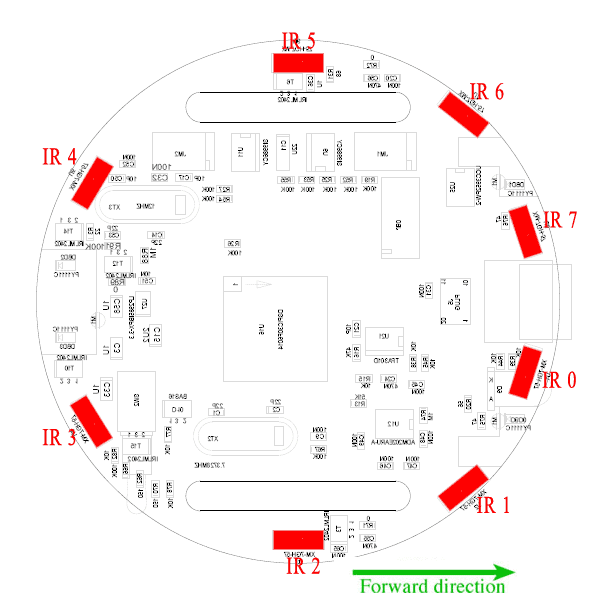
\includegraphics[scale=0.2]{proximity_emplacement.png}
        \end{column}
    \end{columns}
\end{frame}

\begin{frame}
    \frametitle{Akcelerometr}
    \begin{columns}
        \begin{column}{0.6\textwidth}
            \begin{itemize}
                \item 3D akcelerometr
                \item Z robota se dá získat:
                    \begin{itemize}
                        \item Vektor akcelerace
                        \item Zpracované informace (rotace, zrychlení, \ldots)
                    \end{itemize}
                \item Detekce nárazu, naklonění, směru pohybu
            \end{itemize}
        \end{column}

        \begin{column}{0.4\textwidth}
            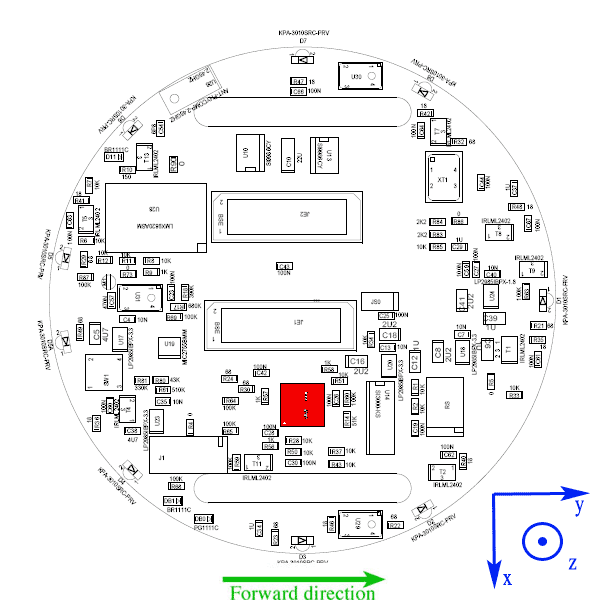
\includegraphics[scale=0.2]{acc_emplacement.png}
        \end{column}
    \end{columns}
\end{frame}

\begin{frame}
    \frametitle{Mikrofony}
    \begin{columns}
        \begin{column}{0.6\textwidth}
            \begin{itemize}
                \item 3D akcelerometr
                \item Z robota se dá získat:
                    \begin{itemize}
                        \item Vektor akcelerace
                        \item Zpracované informace (rotace, zrychlení, \ldots)
                    \end{itemize}
                \item Detekce nárazu, naklonění, směru pohybu
            \end{itemize}
        \end{column}

        \begin{column}{0.4\textwidth}
            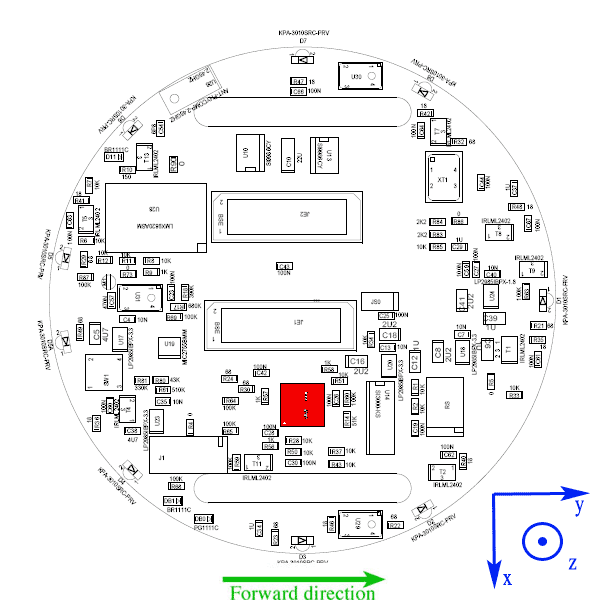
\includegraphics[scale=0.2]{acc_emplacement.png}
        \end{column}
    \end{columns}
\end{frame}

\section{Připojení}

\begin{frame}[t]
    \begin{itemize}
        \item Pokus
    \end{itemize}
\end{frame}

\section{Komunikace}

\begin{frame}
    \begin{itemize}
        \item Pokus
    \end{itemize}
\end{frame}

\subsection{Synchronní}

\begin{frame}
    \begin{itemize}
        \item Pokus
    \end{itemize}
\end{frame}

\subsection{Asynchronní}

\begin{frame}
    \begin{itemize}
        \item Pokus
    \end{itemize}
\end{frame}

\section{Přehled příkazů}

\begin{frame}
    \begin{itemize}
        \item Pokus
    \end{itemize}
\end{frame}

\section{Ukázky programů}

\begin{frame}
    \begin{itemize}
        \item Pokus
    \end{itemize}
\end{frame}


\end{document}
